\subsection{Particle Identification}

Now that things are clustered properly, we move on to do particle identification like in figure \ref{pidEvent}.

\begin{figure}[H]
  % OWN
  \centering
  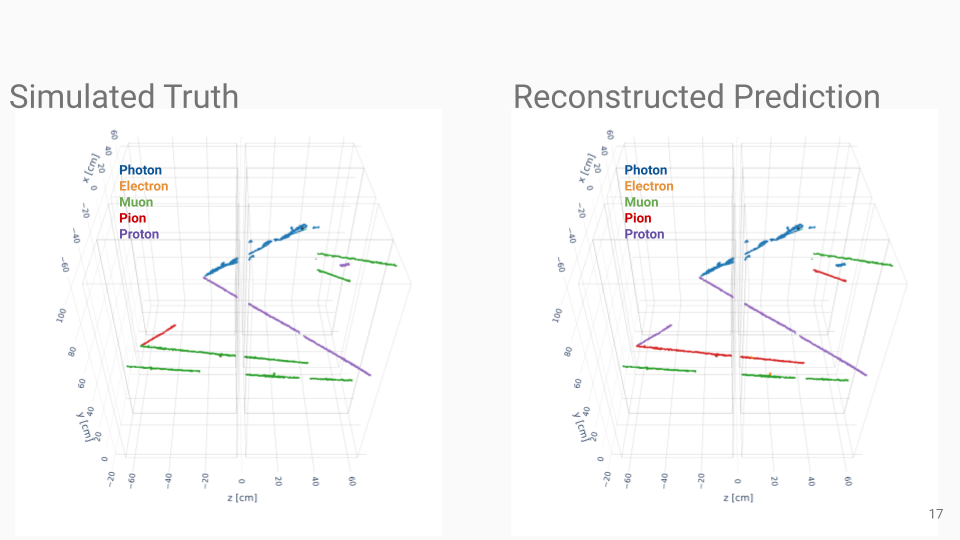
\includegraphics[width=120mm]{figures/pidEvent.png}
  \caption{Particle ID Event display comparing monte carlo truth and reconstructed prediction}
  \label{pidEvent}
\end{figure}

This is done through the Graph Partitioning and Aggregation (GrapPa) GNN.GrapPa innovates by combining partitioning and aggregation techniques to handle massive graphs efficiently.
It first partitions the input graph into smaller, manageable subgraphs, ensuring that computational resources are allocated more effectively.
These partitions are then processed independently through GNN layers, which helps in capturing local graph structures without overwhelming the system's memory.
The aggregation step combines the results from these subgraphs, allowing the model to capture global dependencies and maintain a comprehensive understanding of the entire graph's topology.
This approach strikes a balance between efficiency and expressiveness, making it particularly useful for applications with large and complex graph data.

The GrapPa framework also integrates advanced techniques such as hierarchical pooling and dynamic batching to further enhance its scalability and performance.
Hierarchical pooling enables the model to learn and propagate information across different levels of graph granularity, while dynamic batching adjusts the processing load according to the current computational demands.
These features contribute to GrapPa's ability to generalize well across various graph sizes and structures, addressing key limitations of traditional GNNs which often struggle with scalability and efficiency.

\begin{figure}[H]
  % OWN
  \centering
  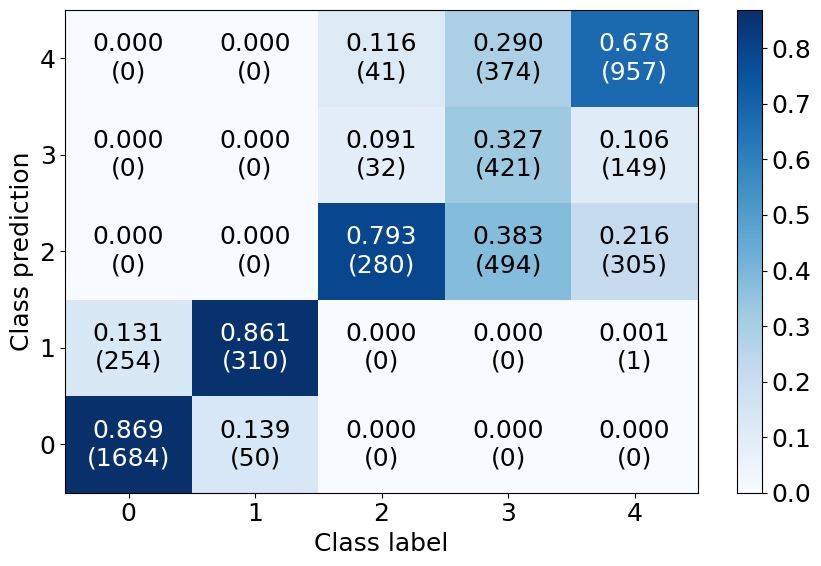
\includegraphics[width=120mm]{figures/pidPerformance.png}
  \caption{Confusion Matrix showing performance of Particle Identification}
  \label{pidPerformance}
\end{figure}

GrapPa tries not only to identify the individual particles but also runs a binary classifier to see if the particle is a primary or secondary.
It is doing a relatively good job at differentiating between different particles with the obvious exception of confusing the pions and muons.
This is because there were so few of them  in the training dataset that identification was difficult and this is expected to improve with more training.

I worked on training and optimizing these models to improve both accuracy and speed of training.
I trained these models on 2x2 simulated data , whereas before it was trained on a generic particle bomb not taking detector geometry or effects into account.
This work allows for better classification of neutrino events in DUNE which is incredibly important for physics analysis when DUNE comes online and starts gathering data.